% ---------------------------------------------------------------------------
% Tarea 3 --- Ajuste de parámetros con Diseño de Experimentos (DOE)
% Compilar con: pdflatex reporte_tarea3.tex  (dos veces)
% ---------------------------------------------------------------------------
\documentclass[11pt,letterpaper]{article}

% ---------- Codificación e idioma ----------
\usepackage[utf8]{inputenc}
\usepackage[spanish,es-nodecimaldot]{babel}

% babel-spanish usa «Cuadro» para las tablas; en este reporte se usa «Tabla».
\addto\captionsspanish{\renewcommand{\tablename}{Tabla}}

% ---------- Matemáticas y gráficos ----------
\usepackage{amsmath,amssymb}
\usepackage{graphicx}

% ---------- Tablas ----------
\usepackage{booktabs}
\usepackage{array}
\usepackage{tabularx}

% ---------- Figuras y listados ----------
\usepackage{float}
\usepackage{caption}
\usepackage{listings}
\usepackage{enumitem}
\usepackage{needspace}
\usepackage{etoolbox}

% ---------- Diseño de página ----------
\usepackage[margin=2.5cm]{geometry}
\usepackage{xcolor}
\usepackage{fancyhdr}
\usepackage{titlesec}
\usepackage[protrusion=true,expansion=true]{microtype}

% ---------- Enlaces y metadatos ----------
\usepackage{hyperref}
\hypersetup{
  colorlinks=true,
  linkcolor=azul,
  urlcolor=azul,
  citecolor=azul,
  pdftitle={Tarea 3: Ajuste de parámetros con Diseño de Experimentos (DOE)},
  pdfauthor={Sebastián Calderón Carrillo},
  pdfsubject={Ajuste de la temperatura inicial del Recocido Simulado con 2-opt sobre el TSP},
}

% ---------- Colores ----------
\definecolor{azul}{HTML}{1F3A5F}
\definecolor{griscodigo}{HTML}{555555}

% ---------- Encabezado y pie ----------
\pagestyle{fancy}
\fancyhf{}
\fancyhead[L]{\small\itshape Tarea 3 --- DOE en Recocido Simulado}
\fancyhead[R]{\small\itshape Algoritmia y Optimización}
\fancyfoot[C]{\small\thepage}
\renewcommand{\headrulewidth}{0.4pt}
\fancypagestyle{primera}{%
  \fancyhf{}%
  \fancyfoot[C]{\small\thepage}%
  \renewcommand{\headrulewidth}{0pt}%
}

% ---------- Títulos ----------
\titleformat{\section}[block]
  {\normalfont\large\bfseries\color{azul}}
  {\thesection.}{0.6em}{}
  [\vspace{2pt}{\color{azul!45}\titlerule[0.6pt]}]
\titlespacing*{\section}{0pt}{2.2ex plus 1ex minus .2ex}{1.1ex plus .2ex}

\titleformat{\subsection}
  {\normalfont\normalsize\bfseries\color{azul!85!black}}
  {\thesubsection}{0.6em}{}
\titlespacing*{\subsection}{0pt}{1.8ex plus .8ex minus .2ex}{0.7ex plus .2ex}

% ---------- Listas ----------
% Se usa el bullet matemático (CMSY10, Type 1) en lugar de \textbullet,
% que en OT1 recurre a una fuente EC bitmap.
\renewcommand{\labelitemi}{\raisebox{0.15ex}{$\bullet$}}
\renewcommand{\labelitemii}{$\circ$}
\setlist[itemize]{leftmargin=1.5em, topsep=3pt, itemsep=1.5pt, parsep=0pt}
\setlist[enumerate]{leftmargin=1.7em, topsep=3pt, itemsep=1.5pt, parsep=0pt}

% ---------- Captions ----------
\captionsetup{font=small,labelfont=bf,labelsep=period}

% ---------- Código ----------
\lstset{
  basicstyle=\ttfamily\footnotesize,
  keywordstyle=\color{azul}\bfseries,
  commentstyle=\color{griscodigo}\itshape,
  stringstyle=\color{griscodigo},
  frame=single,
  rulecolor=\color{black!25},
  backgroundcolor=\color{black!3},
  xleftmargin=6pt,
  xrightmargin=6pt,
  aboveskip=0.9\baselineskip,
  belowskip=0.9\baselineskip,
  showstringspaces=false,
  breaklines=true,
  columns=fullflexible,
  keepspaces=true,
  extendedchars=true,
}

% ---------- Otros ajustes ----------
% Evita títulos huérfanos al final de una página.
\pretocmd{\section}{\Needspace*{6\baselineskip}}{}{}
\pretocmd{\subsection}{\Needspace*{5\baselineskip}}{}{}
\setlength{\emergencystretch}{1.5em}
\allowdisplaybreaks

\begin{document}

% ===========================================================================
% Portada
% ===========================================================================
\thispagestyle{primera}

\begin{center}
  {\color{azul}\rule{\linewidth}{1.2pt}}\\[1.0em]
  {\LARGE\bfseries\color{azul} Tarea 3}\\[0.55em]
  {\Large\bfseries Ajuste de parámetros con Diseño de Experimentos (DOE)}\\[0.7em]
  {\large\itshape Ajuste de la temperatura inicial del Recocido Simulado\\
   con 2-opt sobre el TSP}\\[1.0em]
  {\color{azul}\rule{\linewidth}{0.6pt}}
\end{center}

\vspace{0.4em}

\begin{center}
  \renewcommand{\arraystretch}{1.35}
  \begin{tabular}{@{}l@{\hspace{3.2em}}l@{}}
    \textbf{Materia:}   & Algoritmia y Optimización \\
    \textbf{Profesor:}  & Dr. José Anastacio Hernández Saldaña \\
    \textbf{Alumno:}    & Sebastián Calderón Carrillo \\
    \textbf{Matrícula:} & 2087472 \\
    \textbf{Grupo:}     & 031 \\
    \textbf{Fecha:}     & 14 de noviembre de 2026 \\
  \end{tabular}
\end{center}

\vspace{0.6em}

\noindent\colorbox{black!5}{%
  \parbox{\dimexpr\linewidth-2\fboxsep}{%
    \small\textbf{Repositorio:} \emph{https://github.com/soyscalderon/Tarea-3-Ajuste-de-Parametros-con-Diseno-de-Experimentos-DOE.git}%
  }%
}

\vspace{1.2em}

% ===========================================================================
\section*{Resumen}
% ===========================================================================

Se ajustó la temperatura inicial $T_0$ del Recocido Simulado con 2-opt de la
Tarea 2 mediante un diseño factorial completo $3 \times 3$ (Opción A). El
factor temperatura tuvo tres niveles (bajo, medio y alto), el bloque fue el
tamaño del TSP ($n = 5, 10, 15$) y se hicieron 10 réplicas por punto de
diseño, para un total de 90 corridas. Los niveles se generaron a partir de un
único valor $r \sim U(0,1)$, obtenido con la matrícula como
semilla: $r = 0.6643924310$. Con el rango $[T_{\min}, T_{\max}] = [0.1, 120]$
resultaron $T_0 = 24.00$, $59.97$ y $95.94$.

El ANOVA de dos factores encontró efectos significativos de temperatura
($F = 22.22$, $p = 2.03\times10^{-8}$), tamaño ($F = 534.82$,
$p = 2.12\times10^{-47}$) e interacción ($F = 7.52$,
$p = 3.35\times10^{-5}$). El nivel bajo ($T_0 \approx 24$) fue el de menor
costo para los tres tamaños. En $n = 5$ los tres niveles llegaron exactamente
al mismo óptimo; en $n = 10$ y $n = 15$ el nivel bajo superó de forma
significativa al medio y al alto. La penalización de usar el nivel alto en
lugar del bajo creció de 0\,\% ($n = 5$) a 22.9\,\% ($n = 10$) y 26.5\,\%
($n = 15$), lo que confirma la interacción: la temperatura importa más cuanto
más grande es el problema.

% ===========================================================================
\section{Objetivo y contexto}
% ===========================================================================

La Tarea 2 implementó un Recocido Simulado con movimientos 2-opt para el
Problema del Agente Viajero (TSP) y comparó dos esquemas de enfriamiento. En
esta tarea se retoma ese algoritmo y se ajusta uno de sus parámetros, la
temperatura inicial $T_0$, usando diseño de experimentos. La pregunta central
es si existe una temperatura que produzca tours de menor costo y si esa
temperatura cambia con el tamaño del problema.

Se eligió la \textbf{Opción A (diseño factorial completo con tres niveles)},
que permite estudiar de forma directa los efectos principales de temperatura y
tamaño, y la interacción entre ambos, mediante un ANOVA de dos factores.

% ===========================================================================
\section{Metodología}
% ===========================================================================

\subsection{Algoritmo reutilizado de la Tarea 2}

No se reimplementó el Recocido Simulado. El script
\texttt{src/6.doe\_temperatura.py} carga
\texttt{src/4.simulated\_annealing.py} y reutiliza:

\begin{itemize}
  \item \texttt{tour\_length}: costo de un tour como suma de distancias
        euclidianas.
  \item \texttt{two\_opt\_neighbor}: movimiento 2-opt que invierte un segmento
        aleatorio.
  \item \texttt{simulated\_annealing}: acepta un vecino peor con probabilidad
        $\exp(-\Delta/T)$ y termina cuando la temperatura llega a cero.
  \item \texttt{linear\_cooling\_schedule}: enfriamiento lineal de $T_0$ a 0.
\end{itemize}

Para que la comparación entre niveles fuera justa, todas las corridas usaron
el mismo esquema de enfriamiento lineal y el mismo presupuesto de
\textbf{3,000 pasos}. Así, la temperatura inicial fue el único parámetro que
cambió entre niveles. Cada corrida partió de un tour inicial aleatorio.

\subsection{Instancias}

Se generó \textbf{una instancia aleatoria por tamaño} en un cuadrado de
$10 \times 10$, con semillas independientes:

\begin{table}[H]
  \centering
  \caption{Instancias usadas en el experimento.}
  \label{tab:instancias}
  \renewcommand{\arraystretch}{1.15}
  \begin{tabular}{@{}ccc@{}}
    \toprule
    Tamaño $n$ & Semilla de instancia & Número de ciudades \\
    \midrule
    5  & 10005 & 5  \\
    10 & 10010 & 10 \\
    15 & 10015 & 15 \\
    \bottomrule
  \end{tabular}
\end{table}

Las 10 réplicas de cada punto de diseño usaron las semillas de corrida
20000 a 20009. Esas mismas 10 semillas se usaron en los tres niveles de
temperatura (números aleatorios comunes), de modo que las diferencias entre
temperaturas no se confundieran con la elección del tour inicial ni con la
secuencia aleatoria del algoritmo.

\subsection{Generación de los niveles de temperatura}

Se generó un solo valor $r$ al inicio del experimento, con la matrícula como
semilla:

\begin{lstlisting}[language=Python]
SEMILLA_MATRICULA = 2087472
r = random.Random(SEMILLA_MATRICULA).random()   # r = 0.6643924310
\end{lstlisting}

El valor se usó durante todo el experimento y no se volvió a generar. Se
definió el rango $[T_{\min}, T_{\max}] = [0.1, 120]$ y se aplicaron las
fracciones de la Opción A:

\begin{table}[H]
  \centering
  \caption{Niveles de temperatura inicial generados con la Opción A.}
  \label{tab:niveles}
  \renewcommand{\arraystretch}{1.15}
  \begin{tabular}{@{}ccc@{}}
    \toprule
    Nivel & Fracción & $T_0$ real \\
    \midrule
    bajo  & $0.3r = 0.199318$        & 24.00 \\
    medio & $0.3r + 0.3 = 0.499318$  & 59.97 \\
    alto  & $0.3r + 0.6 = 0.799318$  & 95.94 \\
    \bottomrule
  \end{tabular}
\end{table}

La conversión fue $T_{\text{nivel}} = T_{\min} + \text{fracción} \cdot
(T_{\max} - T_{\min})$.

\subsection{Diseño experimental y modelo}

El diseño es un factorial $3 \times 3$ con 10 réplicas por celda:

\begin{table}[H]
  \centering
  \caption{Diseño factorial $3 \times 3$ con 10 réplicas por celda.}
  \label{tab:diseno}
  \renewcommand{\arraystretch}{1.15}
  \begin{tabular}{@{}cccc@{}}
    \toprule
    Temperatura & $n = 5$ & $n = 10$ & $n = 15$ \\
    \midrule
    bajo (24.00)  & 10 & 10 & 10 \\
    medio (59.97) & 10 & 10 & 10 \\
    alto (95.94)  & 10 & 10 & 10 \\
    \bottomrule
  \end{tabular}
\end{table}

El modelo ANOVA de dos factores con interacción fue:

\[
  \text{costo}_{ijk} = \mu + \tau_i + \beta_j + (\tau\beta)_{ij}
  + \varepsilon_{ijk},
\]

donde $\tau_i$ es el efecto del nivel de temperatura $i$, $\beta_j$ el efecto
del tamaño $j$, $(\tau\beta)_{ij}$ la interacción y $\varepsilon_{ijk}$ el
error aleatorio. Se ajustó con \texttt{statsmodels}:

\begin{lstlisting}[language=Python]
modelo = ols("costo ~ C(temperatura_nivel) * C(tamano)", data=datos).fit()
tabla_anova = sm.stats.anova_lm(modelo, typ=2)
\end{lstlisting}

Se usó $\alpha = 0.05$ (95\,\% de confianza). Para cada efecto se contrasta
$H_0$: el efecto no es significativo, contra $H_1$: sí lo es.

\subsection{Bootstrap de la mediana}

Para cada uno de los 9 puntos de diseño se calcularon la mediana y un
intervalo de confianza del 95\,\% por bootstrap, con 10,000 remuestreos con
reemplazo de las 10 réplicas. Se usó el método de percentiles (2.5\,\% y
97.5\,\%). Como los tres efectos del ANOVA resultaron significativos, el
bootstrap se reporta para los 9 puntos de diseño.

% ===========================================================================
\section{Resultados}
% ===========================================================================

\subsection{ANOVA de dos factores}

La tabla completa es:

\begin{table}[H]
  \centering
  \caption{ANOVA de dos factores con interacción.}
  \label{tab:anova}
  \footnotesize
  \setlength{\tabcolsep}{6pt}
  \renewcommand{\arraystretch}{1.2}
  \begin{tabular}{@{}lrrrrrr@{}}
    \toprule
    Fuente & Suma de cuadrados & gl & Cuadrado medio & $F$ & $p$-valor & $\eta^2$ \\
    \midrule
    Temperatura           & 427.220    & 2 & 213.610   & 22.215  & $2.03\times10^{-8}$  & 0.0363 \\
    Tamaño                & 10,285.172 & 2 & 5,142.586 & 534.824 & $2.12\times10^{-47}$ & 0.8731 \\
    Temperatura $\times$ Tamaño & 289.092 & 4 & 72.273 & 7.516 & $3.35\times10^{-5}$ & 0.0245 \\
    Error                 & 778.853    & 81 & 9.615    & ---     & ---                  & 0.0661 \\
    \bottomrule
  \end{tabular}

  \vspace{2pt}
  \begin{minipage}{\linewidth}
    \footnotesize gl: grados de libertad.
  \end{minipage}
\end{table}

Los tres efectos son significativos con $\alpha = 0.05$:

\begin{itemize}
  \item \textbf{Temperatura:} $F(2,81) = 22.22$, $p = 2.03\times10^{-8}$.
  \item \textbf{Tamaño:} $F(2,81) = 534.82$, $p = 2.12\times10^{-47}$.
  \item \textbf{Interacción:} $F(4,81) = 7.52$, $p = 3.35\times10^{-5}$.
\end{itemize}

El tamaño explica la mayor parte de la variación ($\eta^2 = 0.873$), lo cual
es esperable: un TSP de 15 ciudades tiene un costo mucho mayor que uno de 5.
La temperatura explica 3.6\,\% y la interacción 2.5\,\%, pero ambas son
estadísticamente significativas. La interacción indica que el efecto de la
temperatura \textbf{no es el mismo} en los tres tamaños.

\subsection{Efectos principales}

\begin{figure}[H]
  \centering
  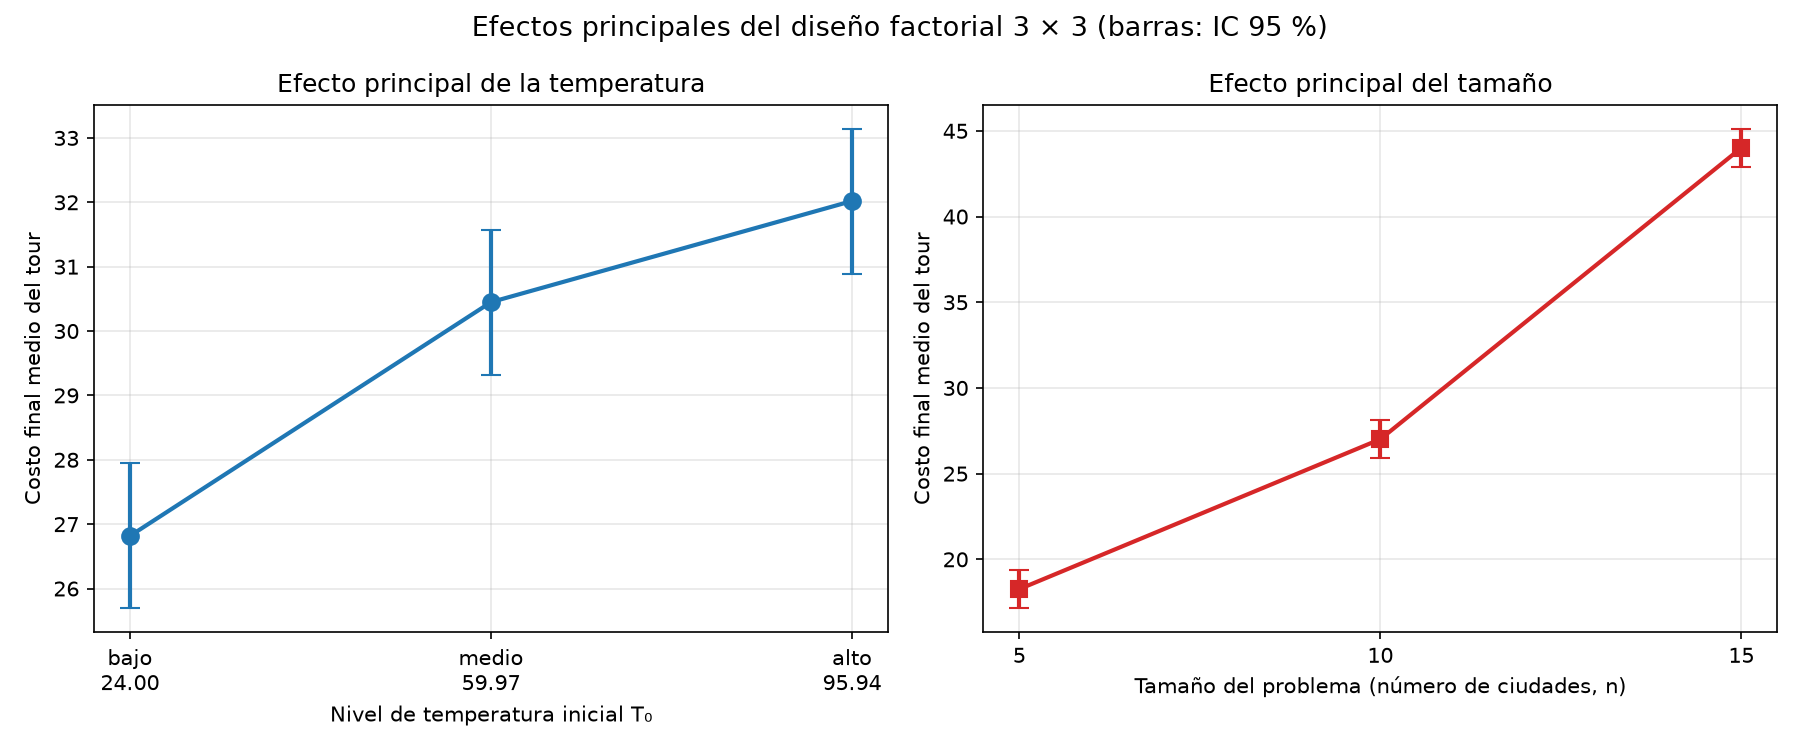
\includegraphics[width=0.92\linewidth]{../graphs/6.doe_efectos_principales.png}
  \caption{Efectos principales de temperatura y tamaño. Las barras son
  intervalos de confianza del 95\,\% calculados con el cuadrado medio del error
  del ANOVA.}
  \label{fig:efectos}
\end{figure}

En la gráfica de efectos principales (Figura~\ref{fig:efectos}) se observa que
el costo medio aumenta al pasar de temperatura baja a media y alta. El
promedio marginal pasa de 26.82 con el nivel bajo a 30.45 con el medio y 32.02
con el alto. El efecto del tamaño es mucho más marcado: 18.26 ($n = 5$), 27.01
($n = 10$) y 44.01 ($n = 15$). La media general es 29.76.

\subsection{Interacción temperatura \texorpdfstring{$\times$}{x} tamaño}

La interacción se ve claramente en la forma de las líneas
(Figura~\ref{fig:interaccion}):

\begin{itemize}
  \item Para $n = 5$ la línea es plana: los tres niveles llegan exactamente al
        mismo costo medio, 18.264.
  \item Para $n = 10$ el costo sube de 24.176 (bajo) a 27.143 (medio) y 29.716
        (alto): aumentos de 12.3\,\% y 22.9\,\% respecto al nivel bajo.
  \item Para $n = 15$ el costo sube de 38.014 (bajo) a 45.941 (medio) y 48.081
        (alto): aumentos de 20.9\,\% y 26.5\,\%.
\end{itemize}

Es decir, la temperatura es irrelevante cuando el problema es pequeño, pero
su efecto es grande y creciente cuando el problema es más difícil.

\begin{figure}[t]
  \centering
  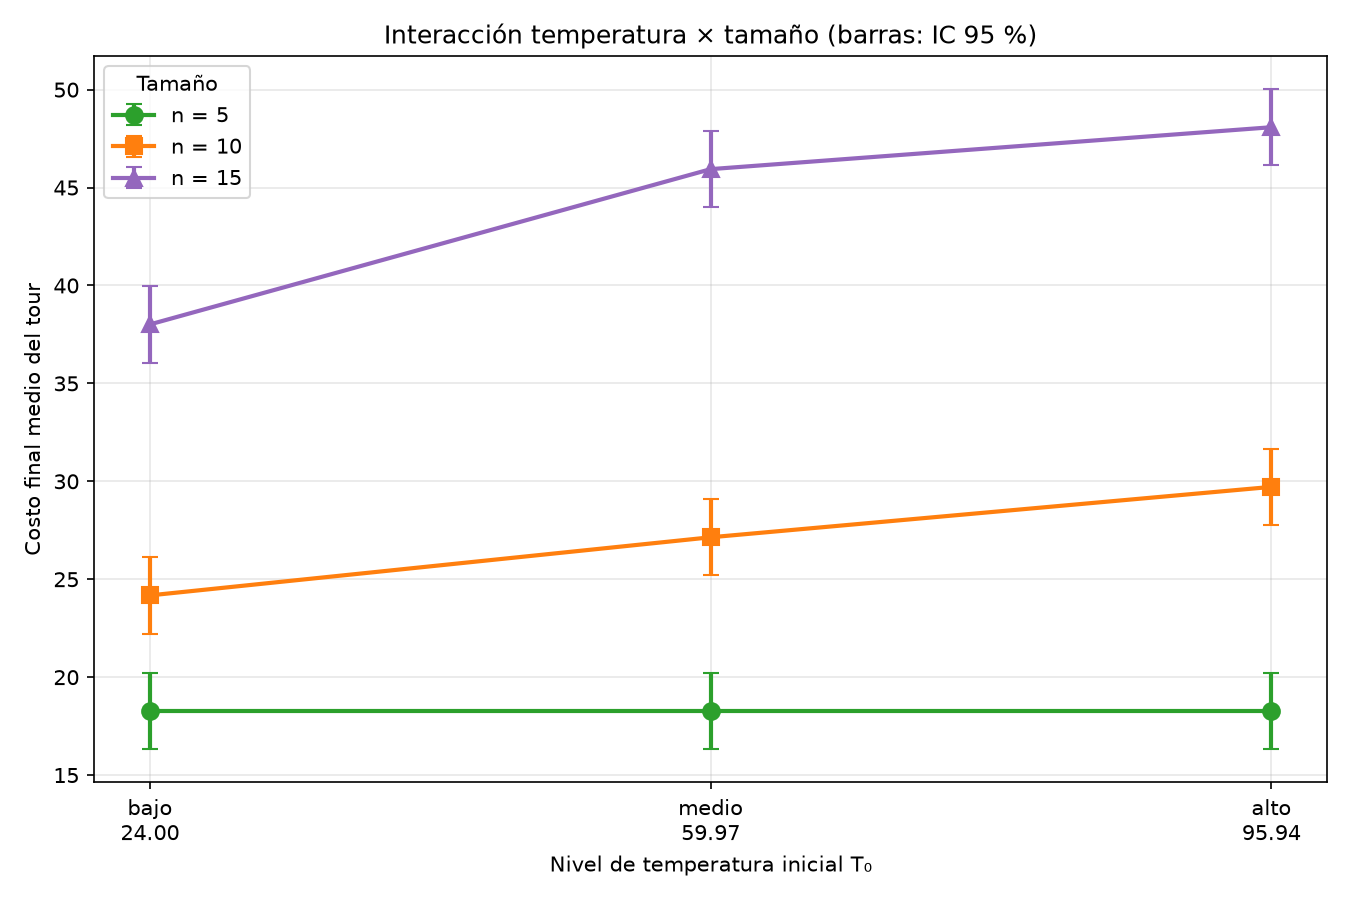
\includegraphics[width=0.70\linewidth]{../graphs/6.doe_interaccion.png}
  \caption{Interacción temperatura $\times$ tamaño. Las líneas no son
  paralelas: el efecto de la temperatura crece con el tamaño del problema.}
  \label{fig:interaccion}
\end{figure}

\subsection{Mediana bootstrap por punto de diseño}

En $n = 5$ las 30 corridas alcanzaron exactamente el mismo tour óptimo, por
eso la desviación y el intervalo son cero. No es un error: significa que el
problema es tan pequeño que el Recocido Simulado siempre lo resuelve, sin
importar la temperatura inicial.

En $n = 10$ el intervalo del nivel bajo no se solapa con el del medio ni con
el del alto. En $n = 15$ el intervalo del nivel bajo (hasta 41.03) queda por
debajo de los intervalos del medio (desde 42.18) y del alto (desde 45.23).
Los niveles medio y alto se solapan entre sí, así que no hay evidencia de que
uno sea mejor que el otro; ambos son peores que el bajo.

\begin{table}[H]
  \centering
  \caption{Mediana bootstrap e intervalo de confianza del 95\,\% por punto de
  diseño.}
  \label{tab:bootstrap}
  \small
  \setlength{\tabcolsep}{5pt}
  \renewcommand{\arraystretch}{1.15}
  \begin{tabular}{@{}cccccc@{}}
    \toprule
    $n$ & Nivel & $T_0$ & Media $\pm$ DE & Mediana bootstrap & IC 95\,\% \\
    \midrule
    5  & bajo  & 24.00 & $18.26 \pm 0.00$ & 18.26 & $[18.26,\, 18.26]$ \\
    5  & medio & 59.97 & $18.26 \pm 0.00$ & 18.26 & $[18.26,\, 18.26]$ \\
    5  & alto  & 95.94 & $18.26 \pm 0.00$ & 18.26 & $[18.26,\, 18.26]$ \\
    10 & bajo  & 24.00 & $24.18 \pm 0.43$ & 24.04 & $[24.04,\, 24.04]$ \\
    10 & medio & 59.97 & $27.14 \pm 2.02$ & 27.11 & $[25.41,\, 28.77]$ \\
    10 & alto  & 95.94 & $29.72 \pm 3.58$ & 29.68 & $[27.06,\, 32.65]$ \\
    15 & bajo  & 24.00 & $38.01 \pm 3.48$ & 38.11 & $[34.44,\, 41.03]$ \\
    15 & medio & 59.97 & $45.94 \pm 5.12$ & 47.07 & $[42.17,\, 49.72]$ \\
    15 & alto  & 95.94 & $48.08 \pm 5.58$ & 46.75 & $[45.23,\, 50.12]$ \\
    \bottomrule
  \end{tabular}
\end{table}

\subsection{Tabla resumen: mejor temperatura por tamaño}

\begin{table}[H]
  \centering
  \caption{Mejor temperatura por tamaño del problema.}
  \label{tab:resumen}
  \small
  \setlength{\tabcolsep}{5pt}
  \renewcommand{\arraystretch}{1.15}
  \begin{tabular}{@{}cccccc@{}}
    \toprule
    Tamaño $n$ & Mejor nivel & $T_0$ óptima & Mediana bootstrap & IC 95\,\% & Media $\pm$ DE \\
    \midrule
    5  & bajo & 24.00 & 18.26 & $[18.26,\, 18.26]$ & $18.26 \pm 0.00$ \\
    10 & bajo & 24.00 & 24.04 & $[24.04,\, 24.04]$ & $24.18 \pm 0.43$ \\
    15 & bajo & 24.00 & 38.11 & $[34.44,\, 41.03]$ & $38.01 \pm 3.48$ \\
    \bottomrule
  \end{tabular}
\end{table}

\textbf{Cómo se llegó a esta conclusión.} Primero, el ANOVA mostró que los
efectos de temperatura, tamaño e interacción son significativos
($p < 0.05$). Como la interacción es significativa, el efecto de temperatura
se analizó por tamaño: en $n = 10$ y $n = 15$ el nivel bajo tiene la menor
media y la menor mediana bootstrap; en $n = 5$ los tres niveles empatan.
Segundo, el bootstrap confirma que en $n = 10$ y $n = 15$ el intervalo del
nivel bajo no se solapa con el de los otros dos. Tercero, las pruebas de Tukey
HSD separan al nivel bajo del medio y del alto en $n = 10$ y $n = 15$ (ver
sección 3.6). Por eso se selecciona el nivel bajo, $T_0 = 24.00$, para los
tres tamaños.

\subsection{Pruebas de respaldo por tamaño}

Como el ANOVA supone varianzas homogéneas y en $n = 5$ la varianza es cero, se
agregaron pruebas no paramétricas y comparaciones múltiples por tamaño:

\begin{table}[H]
  \centering
  \caption{Pruebas de Kruskal-Wallis y Tukey HSD por tamaño.}
  \label{tab:posthoc}
  \small
  \renewcommand{\arraystretch}{1.2}
  \begin{tabularx}{\linewidth}{@{}c
      >{\raggedright\arraybackslash}p{4.3cm}
      >{\raggedright\arraybackslash}X@{}}
    \toprule
    $n$ & Kruskal-Wallis & Tukey HSD (comparaciones significativas) \\
    \midrule
    5  & No aplica: las 30 corridas son idénticas.
       & No aplica: varianza cero. \\
    10 & $H = 17.29$, $p = 1.76\times10^{-4}$
       & bajo vs.\ medio: $p = 0.0257$; bajo vs.\ alto: $p = 0.0001$;
         medio vs.\ alto: $p = 0.058$ \\
    15 & $H = 14.44$, $p = 7.30\times10^{-4}$
       & bajo vs.\ medio: $p = 0.0028$; bajo vs.\ alto: $p = 0.0002$;
         medio vs.\ alto: $p = 0.587$ \\
    \bottomrule
  \end{tabularx}
\end{table}

En ambos tamaños el nivel bajo es significativamente mejor que el medio y que
el alto. La diferencia entre medio y alto no es significativa: una vez que la
temperatura es demasiado alta, subirla más no empeora de forma detectable el
resultado, pero tampoco lo mejora.

\subsection{Distribución de los costos}

\begin{figure}[t]
  \centering
  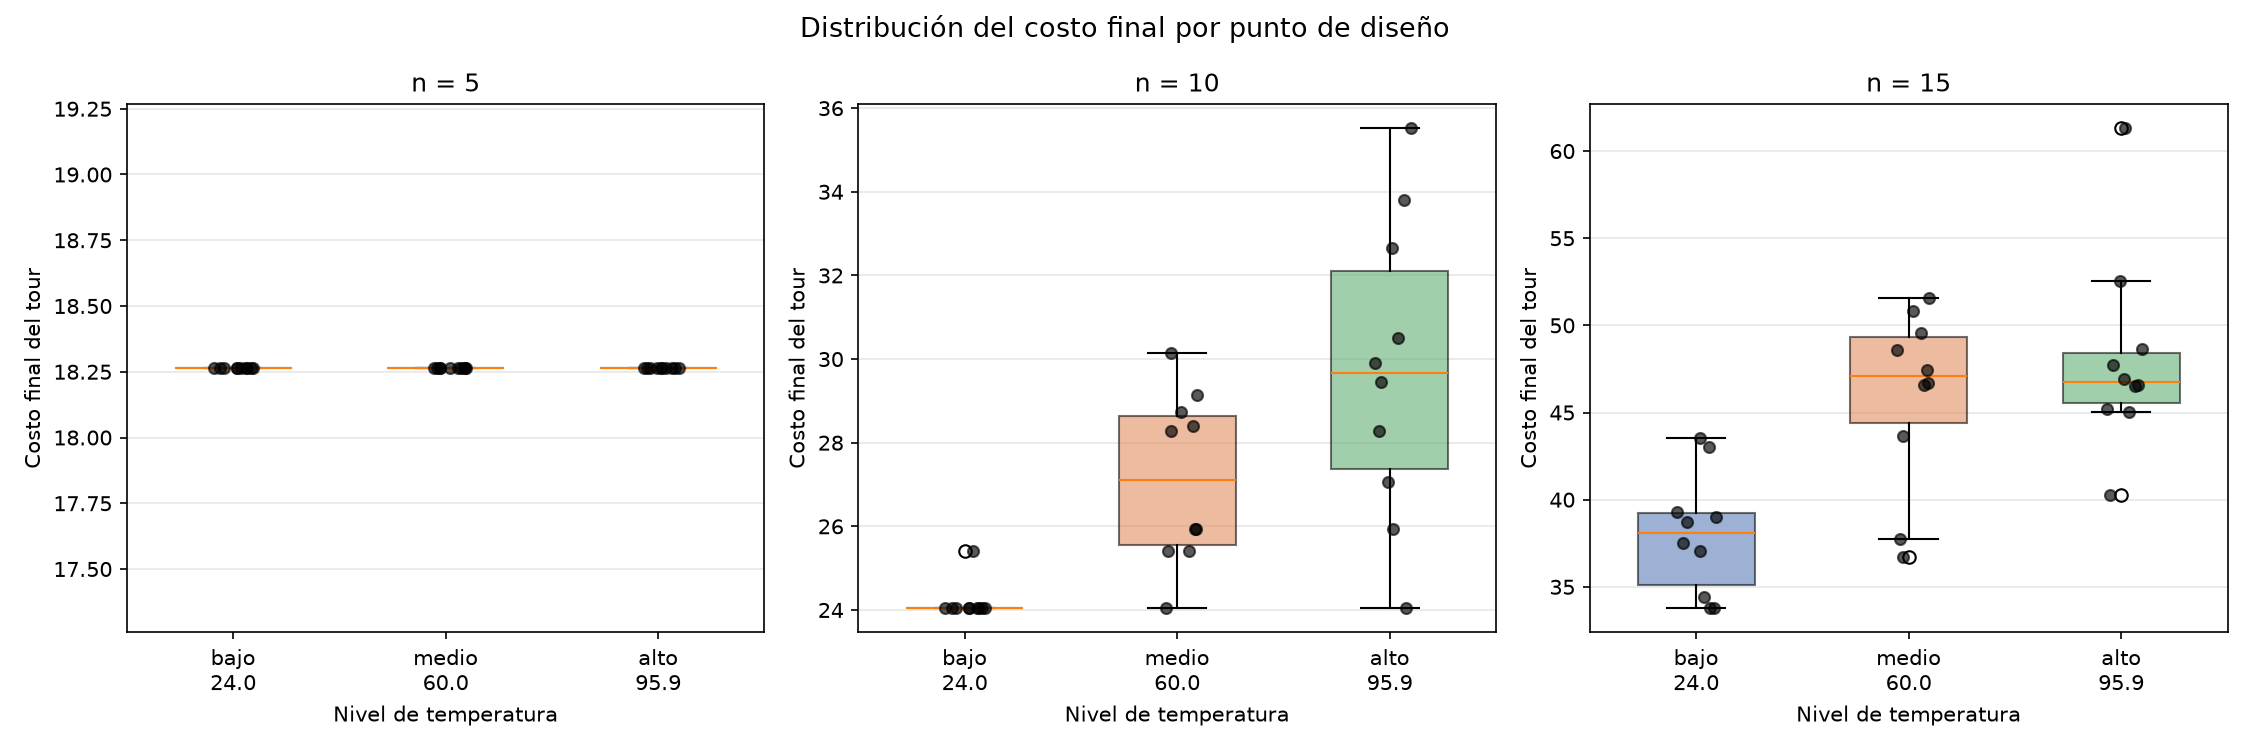
\includegraphics[width=\linewidth]{../graphs/6.doe_distribuciones.png}
  \caption{Distribución del costo final en cada punto de diseño. Cada punto
  negro es una corrida; las cajas resumen la distribución de las 10 réplicas.}
  \label{fig:distribuciones}
\end{figure}

La Figura~\ref{fig:distribuciones} muestra que en $n = 5$ todas las corridas
colapsan en el mismo valor. En $n = 10$ el nivel bajo es muy estable (casi
todas las corridas alcanzan el óptimo), mientras que el medio y el alto tienen
colas hacia costos mayores. En $n = 15$ la dispersión es mayor y el nivel bajo
conserva la mediana más baja, aunque con variabilidad apreciable.

% ===========================================================================
\section{Análisis}
% ===========================================================================

\subsection{¿La temperatura óptima cambia con el tamaño del problema?}

\textbf{No en el nivel seleccionado:} el nivel bajo ($T_0 \approx 24$) es el
mejor para $n = 5$, $10$ y $15$. Lo que cambia con el tamaño es la
\textbf{importancia} de la temperatura, no el valor óptimo dentro de los tres
niveles evaluados. En $n = 5$ los tres niveles empatan porque el espacio de
búsqueda es diminuto y el algoritmo siempre encuentra el óptimo. En $n = 10$ y
$n = 15$ el nivel alto pierde 22.9\,\% y 26.5\,\% de costo frente al bajo,
respectivamente, y el nivel medio pierde 12.3\,\% y 20.9\,\%.

La explicación es el presupuesto fijo de 3,000 pasos. Con una temperatura
inicial alta, el algoritmo pasa muchas iteraciones aceptando movimientos
malos; cuando por fin la temperatura baja, ya no le quedan suficientes pasos
para refinar el tour. En un problema de 5 ciudades eso no importa porque el
2-opt encuentra el óptimo de todas formas; en 15 ciudades sí importa porque
el paisaje tiene más óptimos locales y el tiempo de refinamiento es decisivo.

\subsection{¿Hay una tendencia clara entre \texorpdfstring{$n$}{n} y
\texorpdfstring{$T^*$}{T*}?}

No se observa una tendencia monótona en $T^*$: el mejor nivel es el mismo
para los tres tamaños. Además, como el mejor nivel es el \textbf{límite
inferior} del rango explorado, no se puede afirmar que $T^* = 24$ sea un
óptimo interior; es posible que una temperatura todavía menor produzca un
costo igual o mejor. El experimento solo permite concluir que, entre 24, 60 y
96, la mejor elección es 24.

La tendencia clara está en el \textbf{efecto} de la temperatura: la brecha
entre el nivel bajo y el alto crece con $n$. Esto es exactamente lo que
detecta la interacción significativa del ANOVA.

\subsection{Limitaciones}

\begin{itemize}
  \item \textbf{Una instancia por tamaño:} el enunciado pide una instancia por
        tamaño, así que el efecto de tamaño está confundido con la dificultad
        particular de cada instancia. Las conclusiones sobre $n$ aplican a
        estas instancias.
  \item \textbf{Varianza cero en $n = 5$:} las 30 corridas llegan al mismo
        óptimo. Esto viola levemente el supuesto de homoscedasticidad del
        ANOVA; por eso se reportan Kruskal-Wallis y Tukey como respaldo. Los
        efectos de temperatura e interacción siguen siendo claros en $n = 10$
        y $n = 15$.
  \item \textbf{Presupuesto fijo de 3,000 pasos:} el resultado depende de este
        presupuesto. Con más pasos, el nivel alto podría recuperarse en
        problemas pequeños; con menos pasos, el castigo de una temperatura
        alta sería mayor.
  \item \textbf{Rango de temperatura elegido:} $[0.1, 120]$ es una decisión
        del experimentador. El hecho de que el mejor nivel sea el inferior
        sugiere repetir el experimento con un rango más bajo (por ejemplo,
        $[0.1, 24]$) para localizar el óptimo interior.
  \item \textbf{Bootstrap con 10 réplicas:} los intervalos son anchos,
        especialmente en $n = 15$. Se usan como medida descriptiva de la
        incertidumbre, no como una prueba confirmatoria adicional.
\end{itemize}

% ===========================================================================
\section{Conclusiones}
% ===========================================================================

\begin{enumerate}
  \item El diseño factorial $3 \times 3$ con 90 corridas permitió separar los
        efectos de temperatura, tamaño e interacción. Los tres fueron
        significativos con $\alpha = 0.05$.
  \item El tamaño del problema explica la mayor parte de la variación
        ($\eta^2 = 0.873$), seguido por la temperatura ($\eta^2 = 0.036$) y la
        interacción ($\eta^2 = 0.025$).
  \item La mejor temperatura fue la más baja de las evaluadas, $T_0 = 24.00$,
        para $n = 5$, $10$ y $15$. En $n = 5$ los tres niveles empataron; en
        $n = 10$ y $n = 15$ el nivel bajo fue significativamente mejor que el
        medio y el alto.
  \item La ventaja del nivel bajo crece con el tamaño: la penalización del
        nivel alto frente al bajo fue 0\,\% ($n = 5$), 22.9\,\% ($n = 10$) y
        26.5\,\% ($n = 15$). Por eso la temperatura es un parámetro que
        importa más en instancias grandes.
  \item Para el rango y el presupuesto usados, la recomendación práctica es
        $T_0 \approx 24$ con enfriamiento lineal en 3,000 pasos. Como este
        valor está en el borde inferior del rango, el siguiente experimento
        debería explorar temperaturas menores para verificar si el óptimo es
        aún más bajo.
\end{enumerate}

% ===========================================================================
\section{Reproducibilidad}
% ===========================================================================

El experimento completo se reproduce con:

\begin{lstlisting}[language=bash]
python3 -m venv --system-site-packages .venv
./.venv/bin/pip install -r requirements.txt
./.venv/bin/python src/6.doe_temperatura.py --graph
\end{lstlisting}

Archivos generados:

\begin{itemize}
  \item \texttt{resultados/doe\_temperatura\_corridas.csv}: las 90 corridas.
  \item \texttt{resultados/doe\_temperatura\_anova.csv}: tabla ANOVA.
  \item \texttt{resultados/doe\_temperatura\_posthoc.txt}: Kruskal-Wallis y
        Tukey HSD.
  \item \texttt{resultados/doe\_temperatura\_bootstrap.csv}: medianas e IC por
        punto.
  \item \texttt{resultados/doe\_temperatura\_resumen.csv}: mejor temperatura
        por tamaño.
  \item \texttt{resultados/doe\_temperatura\_metadatos.json}: semillas, $r$,
        niveles y parámetros del experimento.
\end{itemize}

Las gráficas están en \texttt{graphs/} y el código en
\texttt{src/6.doe\_temperatura.py}.

% ===========================================================================
\appendix
\section{Diagnóstico del ANOVA}
% ===========================================================================

\begin{figure}[H]
  \centering
  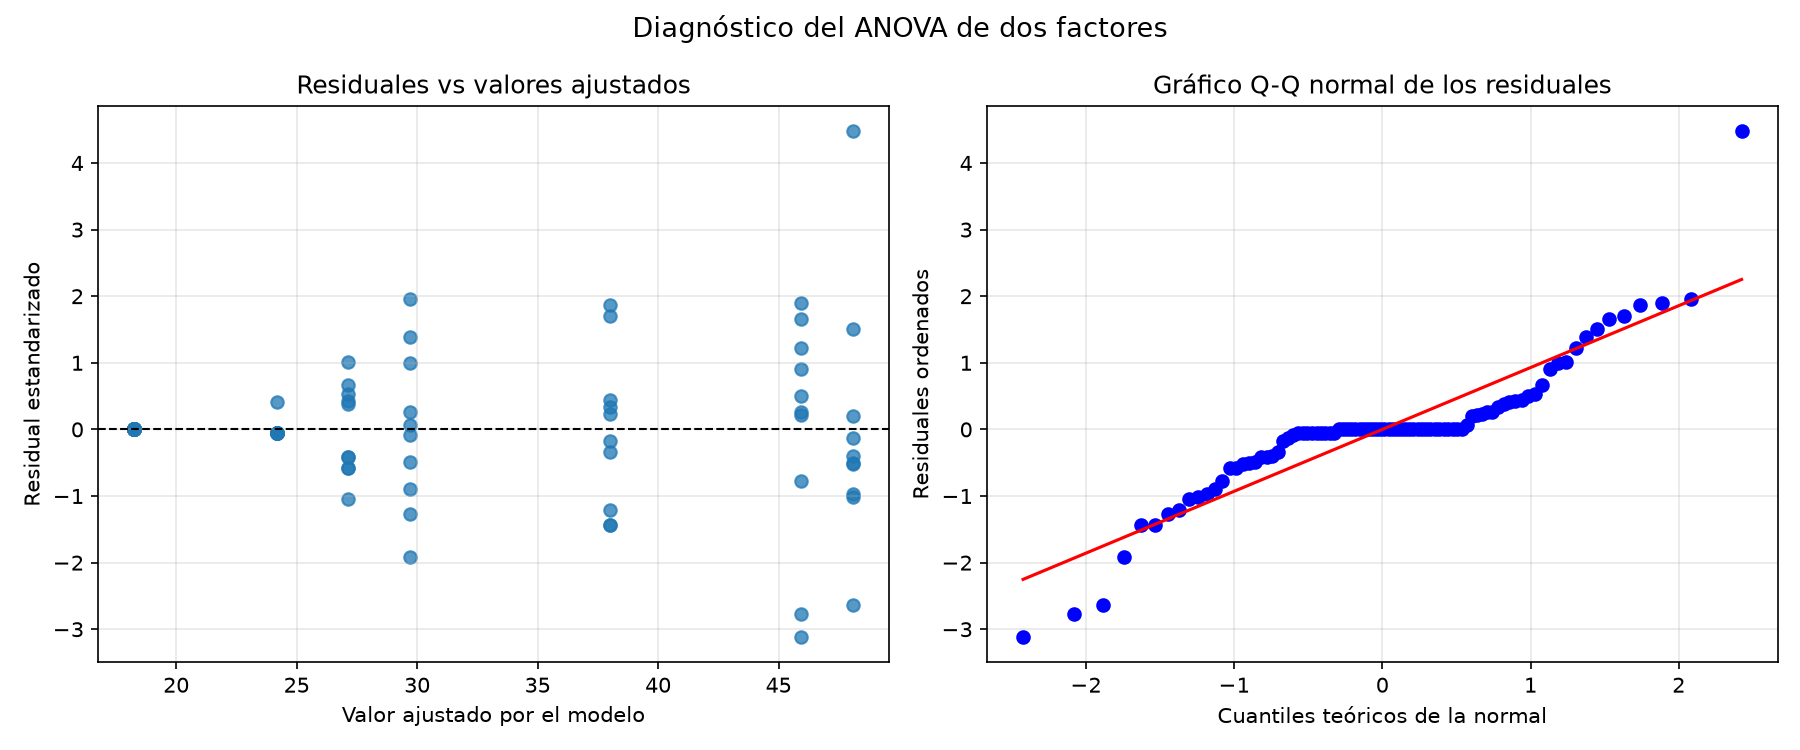
\includegraphics[width=0.92\linewidth]{../graphs/6.doe_diagnostico_anova.png}
  \caption{Residuales del ANOVA. La Q-Q muestra desviaciones en las colas,
  asociadas a la varianza cero de $n = 5$ y a la asimetría de algunas celdas.}
  \label{fig:diagnostico}
\end{figure}

El diagnóstico debe leerse con cautela: la celda $n = 5$ tiene varianza cero,
lo que produce muchos residuales exactamente cero y colas algo pesadas. Aun
así, las pruebas por tamaño (Kruskal-Wallis y Tukey) coinciden con las
conclusiones del ANOVA en $n = 10$ y $n = 15$, que son los tamaños donde la
temperatura tiene un efecto práctico.

\end{document}
